\chapter[CAPÍTULO III]{ANÁLISIS DE LA SITUACIÓN ACTUAL}

\section{Diagrama del Proceso, Mapa de Flujo de Valor y/o Diagrama de Operación actual}

\subsection{Proceso actual de la Empresa - sin la intervención del Software}
El proceso operativo para la atención de requerimientos de soporte técnico, mantenimiento y gestión de inventario en J\&P Periféricos S.A.C. se ejecuta actualmente mediante un flujo empírico y no estandarizado, caracterizado por la dependencia de canales de comunicación informales y registros manuales en hojas de cálculo.

\begin{figure}[H]
    \centering
    \captionsetup{justification=centering}
    \caption{Diagrama de Proceso actual}
    \label{fig:diagrama_proceso_actual}
    \vspace{0.4em}
    
    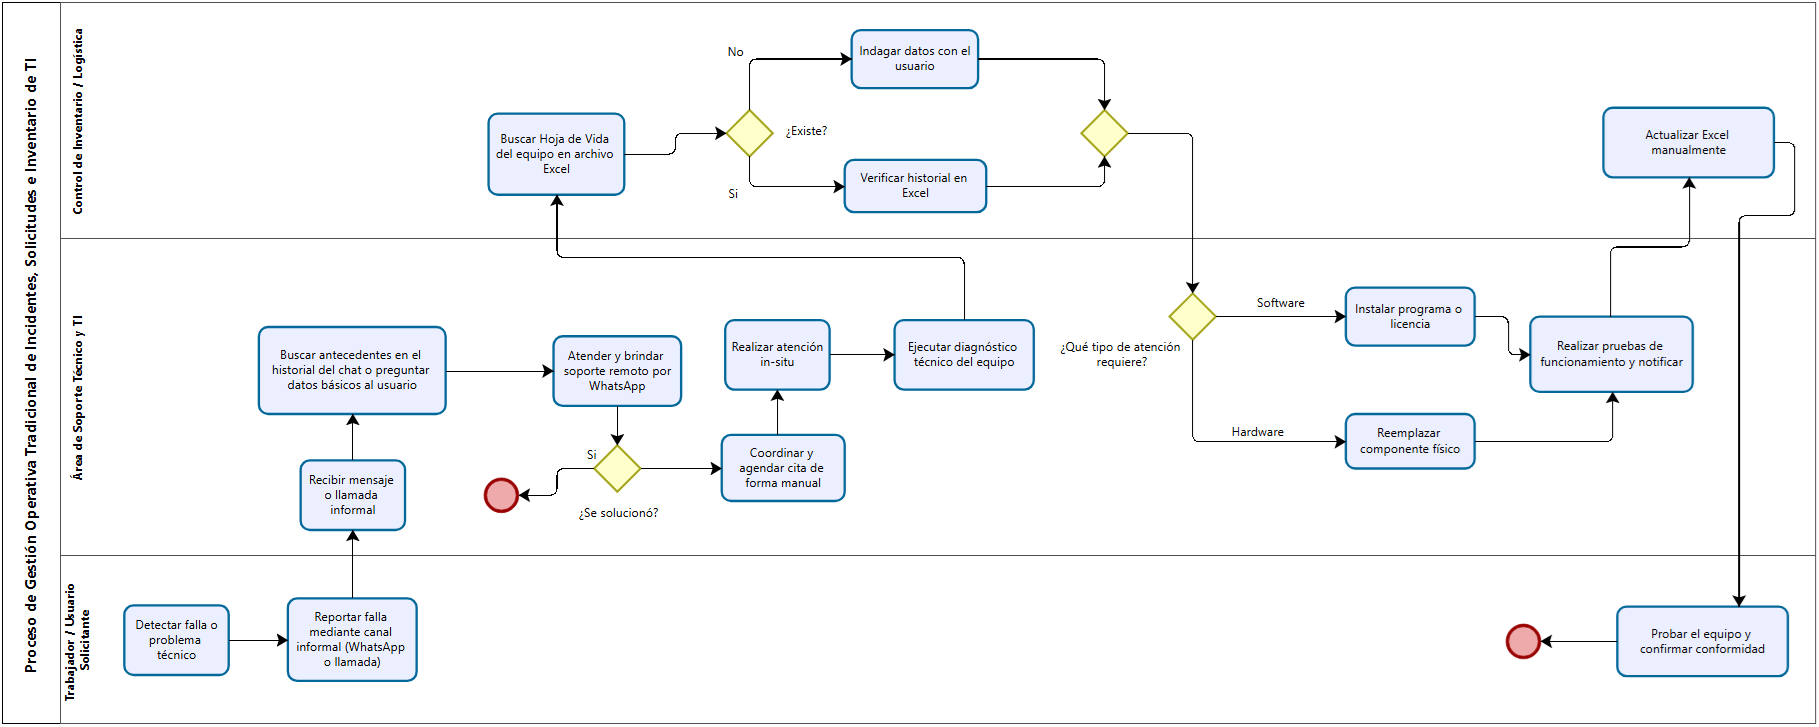
\includegraphics[width=\textwidth]{img/diagrama-proceso-sin-sistema.png}
    
    \vspace{0.4em}
    {\small \textit{Nota.} Representación BPMN del flujo manual de atención y control de inventario antes de la intervención del software.}
\end{figure}

\section{Efecto del Problema en el área del trabajo o en los resultados de la Empresa}

La ausencia de un sistema centralizado de gestión de atenciones técnicas e inventario informático en J\&P Periféricos S.A.C. genera efectos negativos directos que impactan tanto la productividad interna del Área de Soporte Técnico como la satisfacción final de los clientes corporativos.
Para evaluar el impacto de estos efectos en el área de trabajo, se resumen los principales indicadores afectados en la siguiente tabla.

\begingroup
\small
\renewcommand{\arraystretch}{1.15}
\begin{longtable}{@{} c p{13.8cm} @{}}
\caption{Identificación de las Causas del Problema Principal en el Área de Trabajo} \label{tab:causas_problema} \\
\hline
\textbf{N° KPI} & \textbf{IDENTIFICACIÓN DE LAS CAUSAS} \\
\hline
\endfirsthead

\multicolumn{2}{@{}l}{\textbf{Tabla \ref{tab:causas_problema}} \textit{(Continuación)}} \\[0.3em]
\hline
\textbf{N° KPI} & \textbf{IDENTIFICACIÓN DE LAS CAUSAS} \\
\hline
\endhead

\hline
\multicolumn{2}{r}{\textit{Continúa en la siguiente página\dots}} \\
\endfoot

\hline
\multicolumn{2}{@{}p{\textwidth}}{\small \textit{Nota.} Síntesis de las causas operativas identificadas en el diagnóstico del problema principal. Codificación idéntica a la encuesta de priorización (CA1–CA7).} \\
\endlastfoot

CA1 & Búsqueda manual de datos de equipos en archivos Excel desactualizados. \\
\hline
CA2 & Recepción y comunicación por canales informales (WhatsApp/llamadas) sin registro. \\
\hline
CA3 & Descoordinación y reubicación de horarios por cruces en visitas in-situ. \\
\hline
CA4 & Retraso en el escalamiento e identificación del historial de tickets previos. \\
\hline
CA5 & Verificación manual de términos y límites de servicio en contratos (SLA). \\
\hline
CA6 & Elaboración manual de reportes e informes de rendimiento de fin de mes. \\
\hline
CA7 & Carencia de indicadores de rendimiento (KPIs) para evaluar el tiempo de respuesta. \\
\end{longtable}
\endgroup

\section{Análisis de la causa raíz que genera el Problema}
Con la finalidad de identificar las causas fundamentales que originan la desorganización y la falta de trazabilidad en las atenciones técnicas de J\&P Periféricos S.A.C., se aplicó la técnica del Diagrama de Causa-Efecto (Diagrama de Ishikawa). 

\begin{figure}[H]
    \centering
    \captionsetup{justification=centering}
    \caption{Diagrama de Causa-Efecto (Ishikawa) del Problema Principal}
    \label{fig:diagrama_ishikawa}
    \vspace{0.4em}
    
    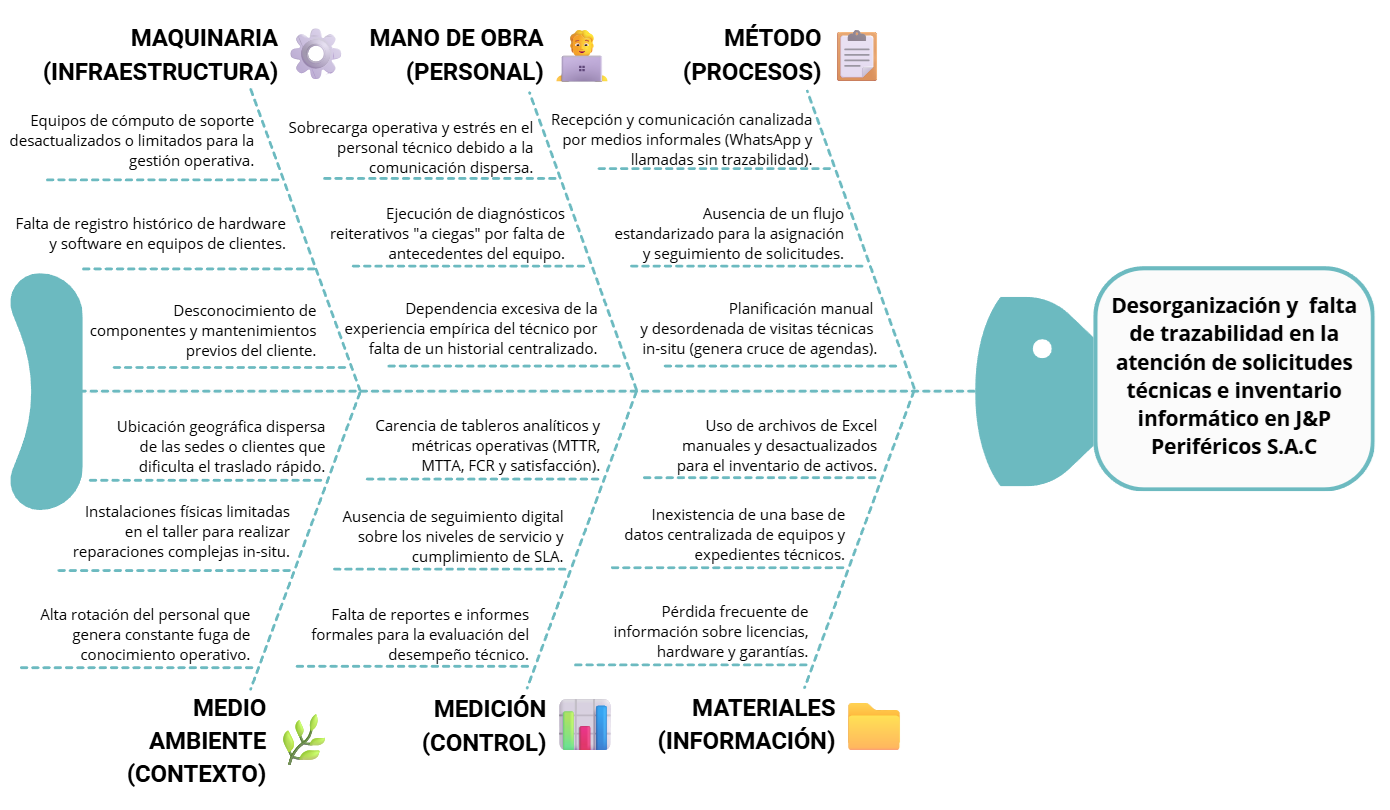
\includegraphics[width=1\textwidth]{img/diagrama_ishikawa.png}
    
    \vspace{0.4em}
    {\small \textit{Nota.} Representación gráfica de las causas raíz agrupadas por categorías de análisis.}
\end{figure}

La estructura de causa-efecto se organiza bajo las seis ramas clásicas del Diagrama de Ishikawa (6M), mapeando explícitamente los códigos CA1–CA7 de la Lista Maestra de Causas conforme al diagrama presentado:

\begin{itemize}[leftmargin=1.27cm]
    \item \textbf{Método (procesos):} CA2 (recepción y comunicación por canales informales sin registro), CA3 (programación empírica de visitas técnicas sin criterio unificado de agenda), CA4 (derivación y escalamiento de incidencias sin flujo estandarizado) y CA5 (verificación manual de términos y límites de servicio en contratos).
    \item \textbf{Mano de Obra (personal):} CA3 (descoordinación y reubicación de horarios por cruces en visitas \textit{in-situ}) y CA4 (retraso en el escalamiento e identificación del historial de tickets previos).
    \item \textbf{Maquinaria (infraestructura):} CA1 (búsqueda manual de datos de equipos en archivos Excel desactualizados), CA2 (falta de plataforma web centralizada para registrar y gestionar tickets) y CA7 (carencia de indicadores de rendimiento KPIs para evaluar el tiempo de respuesta).
    \item \textbf{Materiales (información):} CA1 (búsqueda manual de datos de equipos en archivos Excel desactualizados), CA4 (historial de tickets anteriores no centralizado para consulta rápida) y CA6 (elaboración manual de reportes e informes de rendimiento de fin de mes).
    \item \textbf{Medio Ambiente (contexto):} CA2 (atención fragmentada por mensajería y llamadas en el entorno de servicio) y CA3 (traslados y atención presencial en sedes de clientes sujetas a cambios).
    \item \textbf{Medición (control):} CA5 (verificación manual de términos y límites de servicio en contratos SLA), CA6 (elaboración manual de reportes e informes de rendimiento de fin de mes) y CA7 (carencia de indicadores de rendimiento KPIs para evaluar el tiempo de respuesta).
\end{itemize}

\vspace{0.4em}

\section{Priorización de causa Raíz}
\subsection{Lista de causas encuestadas}
Para evaluar la percepción del personal técnico y operativo respecto al impacto de cada causa raíz identificada, se aplicó un instrumento de encuesta evaluado mediante una escala Likert modificada (4: Muy Crítico / Muy Malo, 3: Crítico / Malo, 2: Regular / Leve, 1: Aceptable / Deficiente) sobre una población de 15 evaluadores.

\begingroup
\footnotesize
\renewcommand{\arraystretch}{1.1}
\begin{longtable}{@{} c p{9.6cm} *{4}{>{\centering\arraybackslash}p{0.6cm}} >{\centering\arraybackslash}p{1.2cm} @{}}
\caption{Resultados de la Encuesta de Valoración de Causas Raíz} \label{tab:encuesta_causas} \\
\hline
\textbf{N°} & \textbf{Identificación de las causas} & \textbf{4} & \textbf{3} & \textbf{2} & \textbf{1} & \textbf{Total Puntaje} \\
\hline
\endfirsthead

\multicolumn{7}{@{}l}{\textbf{Tabla \ref{tab:encuesta_causas}} \textit{(Continuación)}} \\[0.4em]
\hline
\textbf{N°} & \textbf{Identificación de las causas} & \textbf{4} & \textbf{3} & \textbf{2} & \textbf{1} & \textbf{Total Puntaje} \\
\hline
\endhead

\hline
\multicolumn{7}{r}{\textit{Continúa en la siguiente página\dots}} \\
\endfoot

\hline
\multicolumn{7}{@{}p{\textwidth}}{\small \textit{Nota.} Resultados consolidados de las encuestas aplicadas al personal de soporte técnico.} \\
\endlastfoot

CA1 & Búsqueda manual de datos de equipos en archivos Excel desactualizados. & 3 & 7 & 4 & 2 & 43 \\
\hline
CA2 & Recepción y comunicación por canales informales (WhatsApp/llamadas) sin registro. & 3 & 5 & 5 & 2 & 39 \\
\hline
CA3 & Descoordinación y reubicación de horarios por cruces en visitas in-situ. & 2 & 5 & 7 & 2 & 39 \\
\hline
CA4 & Retraso en el escalamiento e identificación del historial de tickets previos. & 2 & 8 & 2 & 1 & 37 \\
\hline
CA5 & Verificación manual de términos y límites de servicio en contratos (SLA). & 2 & 3 & 7 & 3 & 34 \\
\hline
CA6 & Elaboración manual de reportes e informes de rendimiento de fin de mes. & 1 & 3 & 6 & 4 & 29 \\
\hline
CA7 & Carencia de indicadores de rendimiento (KPIs) para evaluar el tiempo de respuesta. & 3 & 2 & 2 & 1 & 23 \\
\hline
\multicolumn{6}{r}{\textbf{Total General:}} & \textbf{244} \\
\end{longtable}
\endgroup

\subsection{Diagrama de Pareto en función al grado de las causas principales}
De acuerdo con la valoración obtenida en las encuestas, se procesaron los datos para construir la distribución acumulada bajo el principio de Pareto (80/20), identificando el grado de incidencia de las causas principales que generan la problemática en el área de soporte técnico de J\&P Periféricos S.A.C. Asimismo, se incluye el esquema de priorización de causa raíz que ilustra de manera directa el impacto de las variables críticas sobre el proceso operativo.

\begin{figure}[H]
    \centering
    \captionsetup{justification=centering}
    \caption{Diagrama de Pareto por Fenómenos}
    \label{fig:diagrama_pareto_por_fenomeno}
    \vspace{0.4em}
    
    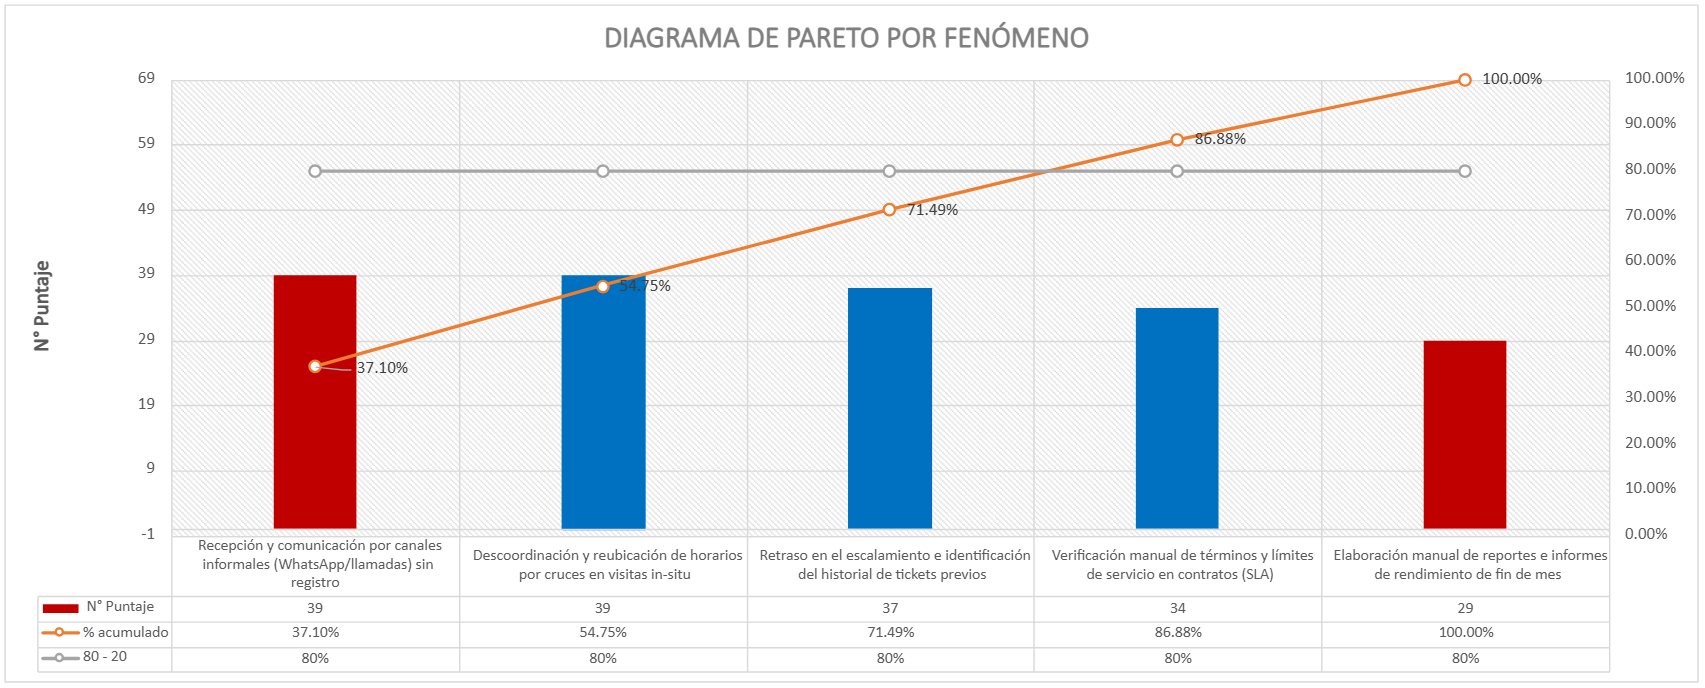
\includegraphics[width=0.95\textwidth]{img/diagrama_pareto_por_fenomeno.png}
    
    \vspace{0.4em}
    {\small \textit{Nota.} Representación gráfica de la distribución acumulada de causas encuestadas en el servicio de soporte técnico.}
\end{figure}

\begin{figure}[H]
    \centering
    \captionsetup{justification=centering}
    \caption{Diagrama de Priorizacion de Causa Raíz}
    \label{fig:diagrama_problema}
    \vspace{0.4em}
    
    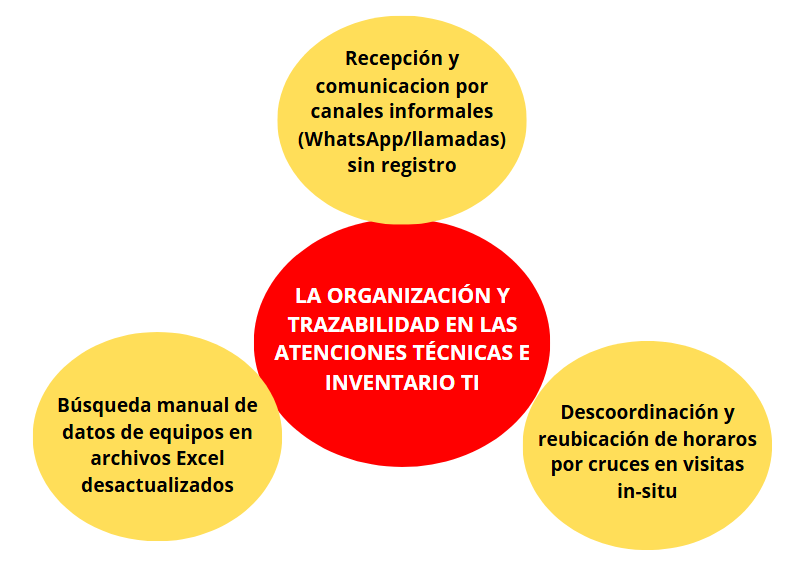
\includegraphics[width=0.95\textwidth]{img/diagrama_problema.png}
    
    \vspace{0.4em}
    {\small \textit{Nota.} Esquema de impacto directo de las causas priorizadas sobre la organizacion y trazabilidad.}
\end{figure}

\subsection{Análisis cualitativo y cuantitativo}

Para evaluar el impacto de cada causa raíz identificada en la encuesta de priorización (Tabla~\ref{tab:encuesta_causas}), se combina el análisis cualitativo del proceso con la cuantificación monetaria del tiempo improductivo operativo en el área de soporte técnico e \textit{in-situ} de J\&P Periféricos S.A.C. durante el período de mayo a septiembre de 2026 (395 atenciones totales y 3 técnicos operativos).

La pérdida económica asociada al tiempo improductivo se determina mediante la siguiente fórmula:

\begin{equation*}
\text{Pérdida Económica (S/)} = N_{\text{eventos}} \times \left(\frac{t_{\text{perdido (min)}}}{60}\right) \times C_{\text{H-H}}
\end{equation*}

donde $N_{\text{eventos}}$ corresponde al número de ocurrencias registradas o identificadas en el período, $t_{\text{perdido (min)}}$ es el tiempo promedio improductivo por ocurrencia expresado en minutos y $C_{\text{H-H}}$ es el costo operativo de hora-hombre del personal de soporte técnico e \textit{in-situ}, fijado internamente en S/ 12.00/hora.

Los datos empleados en el análisis provienen de la observación directa del flujo de atención, la revisión de los registros operativos disponibles (hojas de control, historial de tickets, contratos/SLA y reportes mensuales) y la estimación operativa en campo de los tiempos invertidos en actividades no productivas o repetitivas.

\subsubsection{Causa CA1: Búsqueda manual de datos de equipos en archivos Excel desactualizados}
\noindent \textit{Análisis cualitativo:} El inventario de activos TI y el historial de mantenimiento de los equipos de cómputo por cliente se administran mediante hojas de cálculo en Excel. Al no estar centralizada ni integrada con las solicitudes de atención, los técnicos deben realizar búsquedas manuales de especificaciones, garantías y mantenimientos previos antes o durante cada atención. Esto genera pérdida de tiempo operativo, errores en los diagnósticos y riesgo constante de trabajar con información obsoleta o duplicada. \\

\noindent \textit{Análisis cuantitativo:} 
A partir del registro de atenciones y la observación de búsqueda de activos, se identificaron 103 atenciones con demora por consulta manual en hojas de Excel (26\% del total). Con un tiempo perdido promedio de 25 minutos por incidencia y un costo de S/ 12.00 por hora-hombre (42.92 horas acumuladas), esta causa genera una pérdida económica de S/ 515.00 en el período de mayo a septiembre de 2026.

\begingroup
\small
\renewcommand{\arraystretch}{1.15}
\begin{longtable}{@{} p{4.2cm} >{\centering\arraybackslash}p{2.8cm} >{\centering\arraybackslash}p{2.8cm} >{\centering\arraybackslash}p{1.8cm} >{\centering\arraybackslash}p{2.2cm} @{}}
\caption{Análisis cuantitativo y económico por búsqueda manual de activos (Causa 1)} \label{tab:cuantitativo_causa1} \\
\hline
\textbf{Mes} & \textbf{Atenciones con demora} & \textbf{Total atenciones} & \textbf{Porcentaje} & \textbf{Pérdida estimada (S/)} \\
\hline
\endfirsthead

\multicolumn{5}{@{}l}{\textbf{Tabla \ref{tab:cuantitativo_causa1}} \textit{(Continuación)}} \\[0.4em]
\hline
\textbf{Mes} & \textbf{Atenciones con demora} & \textbf{Total atenciones} & \textbf{Porcentaje} & \textbf{Pérdida estimada (S/)} \\
\hline
\endhead

\hline
\multicolumn{5}{r}{\textit{Continúa en la siguiente página\dots}} \\
\endfoot

\hline
\multicolumn{5}{@{}p{\textwidth}}{\small \textit{Nota.} Registro mensual del impacto operativo y económico por la falta de inventario centralizado ($C_{\text{H-H}} = \text{S/ 12.00/h}$, 25 min por incidencia).} \\
\endlastfoot

May-26 & 18 & 70 & 26\% & S/ 90.00 \\
Jun-26 & 22 & 85 & 26\% & S/ 110.00 \\
Jul-26 & 26 & 95 & 27\% & S/ 130.00 \\
Aug-26 & 16 & 65 & 25\% & S/ 80.00 \\
Sep-26 & 21 & 80 & 26\% & S/ 105.00 \\
\hline
\textbf{Total} & \textbf{103} & \textbf{395} & \textbf{26\% (Prom.)} & \textbf{S/ 515.00} \\
\end{longtable}
\endgroup

\subsubsection{Causa CA2: Recepción y comunicación por canales informales (WhatsApp/llamadas) sin registro}
\noindent \textit{Análisis cualitativo:} La atención de incidentes mediante mensajes de WhatsApp y llamadas telefónicas directas impide registrar de forma oficial el requerimiento, provocando que las solicitudes queden traspapeladas o dispersas en los dispositivos móviles del personal. Esto genera confusión sobre qué técnico atendió a cada cliente, duplicidad en la comunicación y falta de seguimiento formal, ocasionando demoras considerables en el inicio de la atención y una constante pérdida de la trazabilidad operativa. \\

\noindent \textit{Análisis cuantitativo:} 
Mediante el seguimiento de solicitudes recibidas fuera de un canal formal entre mayo y septiembre de 2026, se registraron 149 solicitudes informales (38\% promedio del total de atenciones). Cada atención informal implica un tiempo improductivo promedio de 30 minutos por transcripción, repregunta y seguimiento disperso. Con un costo de S/ 12.00 por hora-hombre (74.50 horas acumuladas), se obtiene una pérdida económica de S/ 894.00 en el período analizado.

\begingroup
\small
\renewcommand{\arraystretch}{1.15}
\begin{longtable}{@{} p{4.2cm} >{\centering\arraybackslash}p{2.8cm} >{\centering\arraybackslash}p{2.8cm} >{\centering\arraybackslash}p{1.8cm} >{\centering\arraybackslash}p{2.2cm} @{}}
\caption{Análisis cuantitativo y económico de solicitudes por canales informales (Causa 2)} \label{tab:cuantitativo_causa2} \\
\hline
\textbf{Mes} & \textbf{Solicitudes informales} & \textbf{Total atenciones} & \textbf{Porcentaje} & \textbf{Pérdida estimada (S/)} \\
\hline
\endfirsthead

\multicolumn{5}{@{}l}{\textbf{Tabla \ref{tab:cuantitativo_causa2}} \textit{(Continuación)}} \\[0.4em]
\hline
\textbf{Mes} & \textbf{Solicitudes informales} & \textbf{Total atenciones} & \textbf{Porcentaje} & \textbf{Pérdida estimada (S/)} \\
\hline
\endhead

\hline
\multicolumn{5}{r}{\textit{Continúa en la siguiente página\dots}} \\
\endfoot

\hline
\multicolumn{5}{@{}p{\textwidth}}{\small \textit{Nota.} Consolidado mensual de incidencia e impacto económico por canales informales ($C_{\text{H-H}} = \text{S/ 12.00/h}$, 30 min por solicitud).} \\
\endlastfoot

May-26 & 26 & 70 & 37\% & S/ 156.00 \\
Jun-26 & 32 & 85 & 38\% & S/ 192.00 \\
Jul-26 & 37 & 95 & 39\% & S/ 222.00 \\
Aug-26 & 24 & 65 & 37\% & S/ 144.00 \\
Sep-26 & 30 & 80 & 38\% & S/ 180.00 \\
\hline
\textbf{Total} & \textbf{149} & \textbf{395} & \textbf{38\% (Prom.)} & \textbf{S/ 894.00} \\
\end{longtable}
\endgroup

\subsubsection{Causa CA3: Descoordinación y reubicación de horarios por cruces en visitas in-situ}
\noindent \textit{Análisis cualitativo:} La programación de visitas presenciales y soporte técnico in-situ en las sedes de los clientes se gestiona de manera manual y sin un calendario centralizado de disponibilidad técnica. Esto provoca cruces de agenda entre los técnicos asignados, reprogramaciones de última hora, tiempos muertos por traslados no optimizados y descoordinación con los horarios de atención de los clientes, lo que afecta la puntualidad y genera insatisfacción en el servicio. \\

\noindent \textit{Análisis cuantitativo:} 
A partir de la revisión de agendas y reprogramaciones de visitas presenciales, se registraron 81 visitas afectadas por cruces de horario (20\% promedio del total). Cada cruce genera un tiempo muerto promedio de 20 minutos de coordinación y reubicación. Valorizado a S/ 12.00 por hora-hombre (27.00 horas acumuladas), esta causa representa una pérdida económica de S/ 324.00 en el período evaluado.

\begingroup
\small
\renewcommand{\arraystretch}{1.15}
\begin{longtable}{@{} p{4.2cm} >{\centering\arraybackslash}p{2.8cm} >{\centering\arraybackslash}p{2.8cm} >{\centering\arraybackslash}p{1.8cm} >{\centering\arraybackslash}p{2.2cm} @{}}
\caption{Análisis cuantitativo y económico de visitas in-situ con reprogramación (Causa 3)} \label{tab:cuantitativo_causa3} \\
\hline
\textbf{Mes} & \textbf{Visitas con cruce de agenda} & \textbf{Total atenciones} & \textbf{Porcentaje} & \textbf{Pérdida estimada (S/)} \\
\hline
\endfirsthead

\multicolumn{5}{@{}l}{\textbf{Tabla \ref{tab:cuantitativo_causa3}} \textit{(Continuación)}} \\[0.4em]
\hline
\textbf{Mes} & \textbf{Visitas con cruce de agenda} & \textbf{Total atenciones} & \textbf{Porcentaje} & \textbf{Pérdida estimada (S/)} \\
\hline
\endhead

\hline
\multicolumn{5}{r}{\textit{Continúa en la siguiente página\dots}} \\
\endfoot

\hline
\multicolumn{5}{@{}p{\textwidth}}{\small \textit{Nota.} Distribución mensual de incidencias y pérdida económica por descoordinación en agenda presencial ($C_{\text{H-H}} = \text{S/ 12.00/h}$, 20 min por visita).} \\
\endlastfoot

May-26 & 14 & 70 & 20\% & S/ 56.00 \\
Jun-26 & 18 & 85 & 21\% & S/ 72.00 \\
Jul-26 & 21 & 95 & 22\% & S/ 84.00 \\
Aug-26 & 12 & 65 & 18\% & S/ 48.00 \\
Sep-26 & 16 & 80 & 20\% & S/ 64.00 \\
\hline
\textbf{Total} & \textbf{81} & \textbf{395} & \textbf{20\% (Prom.)} & \textbf{S/ 324.00} \\
\end{longtable}
\endgroup

\subsubsection{Causa CA4: Retraso en el escalamiento e identificación del historial de tickets previos}
\noindent \textit{Análisis cualitativo:} La falta de un flujo estandarizado para la asignación, seguimiento y escalamiento de tickets impide identificar el historial previo de cada incidencia, generando retrasos en la resolución y pérdida de trazabilidad operativa. Al no existir un registro centralizado de las atenciones anteriores, los técnicos deben re-diagnosticar casos ya atendidos, duplicando esfuerzos y prolongando los tiempos de resolución. \\

\noindent \textit{Análisis cuantitativo:}
Obtuvo un puntaje de 37 en la encuesta de priorización (Tabla~\ref{tab:encuesta_causas}), ubicándose en el cuarto lugar. Según la revisión de casos escalados o reabiertos y la observación del proceso de diagnóstico, se registran 95 casos en los cinco meses (entre 16 y 22 por mes) con un tiempo perdido promedio de 15 minutos por ticket (23.75 horas acumuladas), lo que equivale a una pérdida económica de S/ 285.00.

\begingroup
\small
\renewcommand{\arraystretch}{1.15}
\begin{longtable}{@{} p{4.2cm} >{\centering\arraybackslash}p{2.8cm} >{\centering\arraybackslash}p{2.4cm} >{\centering\arraybackslash}p{2.2cm} >{\centering\arraybackslash}p{2.2cm} @{}}
\caption{Análisis cuantitativo y económico por retraso en escalamiento e historial de tickets (Causa 4)} \label{tab:cuantitativo_causa4} \\
\hline
\textbf{Mes} & \textbf{Tickets afectados} & \textbf{Tiempo / caso (min)} & \textbf{Horas perdidas} & \textbf{Pérdida estimada (S/)} \\
\hline
\endfirsthead

\multicolumn{5}{@{}l}{\textbf{Tabla \ref{tab:cuantitativo_causa4}} \textit{(Continuación)}} \\[0.4em]
\hline
\textbf{Mes} & \textbf{Tickets afectados} & \textbf{Tiempo / caso (min)} & \textbf{Horas perdidas} & \textbf{Pérdida estimada (S/)} \\
\hline
\endhead

\hline
\multicolumn{5}{r}{\textit{Continúa en la siguiente página\dots}} \\
\endfoot

\hline
\multicolumn{5}{@{}p{\textwidth}}{\small \textit{Nota.} Impacto estimado a partir de la revisión de casos escalados/reabiertos y observación operativa ($C_{\text{H-H}} = \text{S/ 12.00/h}$).} \\
\endlastfoot

May-26 & 16 & 15 & 4.00 & S/ 48.00 \\
Jun-26 & 18 & 15 & 4.50 & S/ 54.00 \\
Jul-26 & 20 & 15 & 5.00 & S/ 60.00 \\
Aug-26 & 22 & 15 & 5.50 & S/ 66.00 \\
Sep-26 & 19 & 15 & 4.75 & S/ 57.00 \\
\hline
\textbf{Total} & \textbf{95} & \textbf{15 (Prom.)} & \textbf{23.75} & \textbf{S/ 285.00} \\
\end{longtable}
\endgroup

\subsubsection{Causa CA5: Verificación manual de términos y límites de servicio en contratos (SLA)}
\noindent \textit{Análisis cualitativo:} La verificación de la vigencia de los planes contratados, la cantidad máxima de equipos cubiertos y los tiempos máximos de atención comprometidos se realiza de forma manual y fragmentada, dificultando priorizar oportunamente las incidencias críticas y comprometiendo el cumplimiento de los Acuerdos de Nivel de Servicio (SLA). Esta carencia de control automatizado provoca que se brinde soporte a activos fuera de cobertura y afecte la formalidad del servicio. \\

\noindent \textit{Análisis cuantitativo:}
Obtuvo un puntaje de 34 en la encuesta de priorización (Tabla~\ref{tab:encuesta_causas}), ubicándose en el quinto lugar. A partir del contraste con los documentos de contratos/SLA y la observación de validación previa a la atención, se registran 93 verificaciones manuales en los cinco meses (entre 15 y 23 por mes) con un tiempo promedio de 12 minutos por revisión (18.60 horas acumuladas), generando una pérdida económica de S/ 223.20.

\begingroup
\small
\renewcommand{\arraystretch}{1.15}
\begin{longtable}{@{} p{4.2cm} >{\centering\arraybackslash}p{2.8cm} >{\centering\arraybackslash}p{2.4cm} >{\centering\arraybackslash}p{2.2cm} >{\centering\arraybackslash}p{2.2cm} @{}}
\caption{Análisis cuantitativo y económico por verificación manual de contratos y SLA (Causa 5)} \label{tab:cuantitativo_causa5} \\
\hline
\textbf{Mes} & \textbf{Revisiones SLA} & \textbf{Tiempo / caso (min)} & \textbf{Horas perdidas} & \textbf{Pérdida estimada (S/)} \\
\hline
\endfirsthead

\multicolumn{5}{@{}l}{\textbf{Tabla \ref{tab:cuantitativo_causa5}} \textit{(Continuación)}} \\[0.4em]
\hline
\textbf{Mes} & \textbf{Revisiones SLA} & \textbf{Tiempo / caso (min)} & \textbf{Horas perdidas} & \textbf{Pérdida estimada (S/)} \\
\hline
\endhead

\hline
\multicolumn{5}{r}{\textit{Continúa en la siguiente página\dots}} \\
\endfoot

\hline
\multicolumn{5}{@{}p{\textwidth}}{\small \textit{Nota.} Impacto estimado a partir de la revisión contractual y observación de validación de cobertura ($C_{\text{H-H}} = \text{S/ 12.00/h}$).} \\
\endlastfoot

May-26 & 15 & 12 & 3.00 & S/ 36.00 \\
Jun-26 & 17 & 12 & 3.40 & S/ 40.80 \\
Jul-26 & 20 & 12 & 4.00 & S/ 48.00 \\
Aug-26 & 23 & 12 & 4.60 & S/ 55.20 \\
Sep-26 & 18 & 12 & 3.60 & S/ 43.20 \\
\hline
\textbf{Total} & \textbf{93} & \textbf{12 (Prom.)} & \textbf{18.60} & \textbf{S/ 223.20} \\
\end{longtable}
\endgroup

\subsubsection{Causa CA6: Elaboración manual de reportes e informes de rendimiento de fin de mes}
\noindent \textit{Análisis cualitativo:} La elaboración manual de reportes e informes de rendimiento de fin de mes sobrecarga la operación del área técnica y limita la toma de decisiones basada en datos. Al no existir tableros analíticos automatizados, el personal técnico debe consolidar manualmente la información de atenciones, tiempos y cumplimiento de SLA, consumiendo tiempo que podría destinarse a la atención de incidencias. \\

\noindent \textit{Análisis cuantitativo:}
Obtuvo un puntaje de 29 en la encuesta de priorización (Tabla~\ref{tab:encuesta_causas}), ubicándose en el sexto lugar. Según la revisión de informes mensuales emitidos y la observación del cierre operativo, se elabora 1 reporte consolidado mensual con una dedicación promedio de 4.00 horas por cierre (20.00 horas en cinco meses), lo que representa una pérdida económica de S/ 240.00.

\begingroup
\small
\renewcommand{\arraystretch}{1.15}
\begin{longtable}{@{} p{4.2cm} >{\centering\arraybackslash}p{2.6cm} >{\centering\arraybackslash}p{2.6cm} >{\centering\arraybackslash}p{2.2cm} >{\centering\arraybackslash}p{2.2cm} @{}}
\caption{Análisis cuantitativo y económico por elaboración manual de reportes mensuales (Causa 6)} \label{tab:cuantitativo_causa6} \\
\hline
\textbf{Mes} & \textbf{Reportes emitidos} & \textbf{Horas de cierre} & \textbf{Costo H-H (S/)} & \textbf{Pérdida estimada (S/)} \\
\hline
\endfirsthead

\multicolumn{5}{@{}l}{\textbf{Tabla \ref{tab:cuantitativo_causa6}} \textit{(Continuación)}} \\[0.4em]
\hline
\textbf{Mes} & \textbf{Reportes emitidos} & \textbf{Horas de cierre} & \textbf{Costo H-H (S/)} & \textbf{Pérdida estimada (S/)} \\
\hline
\endhead

\hline
\multicolumn{5}{r}{\textit{Continúa en la siguiente página\dots}} \\
\endfoot

\hline
\multicolumn{5}{@{}p{\textwidth}}{\small \textit{Nota.} Impacto estimado a partir de los informes mensuales elaborados y el tiempo de consolidación de datos.} \\
\endlastfoot

May-26 & 1 & 4.00 & S/ 12.00 & S/ 48.00 \\
Jun-26 & 1 & 4.00 & S/ 12.00 & S/ 48.00 \\
Jul-26 & 1 & 4.00 & S/ 12.00 & S/ 48.00 \\
Aug-26 & 1 & 4.00 & S/ 12.00 & S/ 48.00 \\
Sep-26 & 1 & 4.00 & S/ 12.00 & S/ 48.00 \\
\hline
\textbf{Total} & \textbf{5} & \textbf{20.00} & \textbf{S/ 12.00} & \textbf{S/ 240.00} \\
\end{longtable}
\endgroup

\subsubsection{Causa CA7: Carencia de indicadores de rendimiento (KPIs) para evaluar el tiempo de respuesta}
\noindent \textit{Análisis cualitativo:} La falta de un sistema con backend robusto y modular que centralice las reglas de negocio impide la monitorización en tiempo real de los indicadores de rendimiento y la validación automatizada de contratos, sobrecargando la operación y comprometiendo la calidad del servicio técnico. Sin KPIs como MTTA, MTTR, FCR y CSAT, la gerencia no puede evaluar objetivamente el desempeño del equipo técnico ni el cumplimiento de los SLA. \\

\noindent \textit{Análisis cuantitativo:}
Obtuvo un puntaje de 23 en la encuesta de priorización (Tabla~\ref{tab:encuesta_causas}), ubicándose en el séptimo lugar. A partir de la observación de las actividades de control y seguimiento de tiempos del área, se registra 1 revisión mensual dedicada al control manual de indicadores/tiempos con 2.00 horas por mes (10.00 horas en cinco meses), sin duplicar los tiempos ya contabilizados en las demás causas, lo que equivale a una pérdida económica de S/ 120.00.

\begingroup
\small
\renewcommand{\arraystretch}{1.15}
\begin{longtable}{@{} p{4.2cm} >{\centering\arraybackslash}p{2.6cm} >{\centering\arraybackslash}p{2.6cm} >{\centering\arraybackslash}p{2.2cm} >{\centering\arraybackslash}p{2.2cm} @{}}
\caption{Análisis cuantitativo y económico por carencia de indicadores KPI (Causa 7)} \label{tab:cuantitativo_causa7} \\
\hline
\textbf{Mes} & \textbf{Revisiones / mes} & \textbf{Horas de control} & \textbf{Costo H-H (S/)} & \textbf{Pérdida estimada (S/)} \\
\hline
\endfirsthead

\multicolumn{5}{@{}l}{\textbf{Tabla \ref{tab:cuantitativo_causa7}} \textit{(Continuación)}} \\[0.4em]
\hline
\textbf{Mes} & \textbf{Revisiones / mes} & \textbf{Horas de control} & \textbf{Costo H-H (S/)} & \textbf{Pérdida estimada (S/)} \\
\hline
\endhead

\hline
\multicolumn{5}{r}{\textit{Continúa en la siguiente página\dots}} \\
\endfoot

\hline
\multicolumn{5}{@{}p{\textwidth}}{\small \textit{Nota.} Impacto estimado a partir de la observación de control de tiempos sin duplicar tiempos de otras causas.} \\
\endlastfoot

May-26 & 1 & 2.00 & S/ 12.00 & S/ 24.00 \\
Jun-26 & 1 & 2.00 & S/ 12.00 & S/ 24.00 \\
Jul-26 & 1 & 2.00 & S/ 12.00 & S/ 24.00 \\
Aug-26 & 1 & 2.00 & S/ 12.00 & S/ 24.00 \\
Sep-26 & 1 & 2.00 & S/ 12.00 & S/ 24.00 \\
\hline
\textbf{Total} & \textbf{5} & \textbf{10.00} & \textbf{S/ 12.00} & \textbf{S/ 120.00} \\
\end{longtable}
\endgroup

Con el propósito de cuantificar el impacto financiero que generan las deficiencias operativas detectadas en la gestión de soporte técnico e inventario de TI, se realizó una valorización del tiempo improductivo asociado a cada causa raíz durante el periodo comprendido entre mayo y septiembre de 2026. Para este cálculo se tomó como base un costo hora-hombre de S/ 12.00, permitiendo traducir las horas perdidas en montos acumulados y promedios mensuales concretos. En la \hyperref[tab:consolidado_perdidas_cap3]{Tabla~\ref*{tab:consolidado_perdidas_cap3}} se presenta el consolidado detallado de estas pérdidas económicas desagregadas por cada uno de los siete problemas identificados.

\begingroup
\small
\renewcommand{\arraystretch}{1.15}
\begin{longtable}{@{} c p{8.8cm} >{\centering\arraybackslash}p{2.4cm} >{\centering\arraybackslash}p{2.4cm} @{}}
\caption{Consolidado de pérdidas económicas por causa raíz (mayo – septiembre 2026)} \label{tab:consolidado_perdidas_cap3} \\
\hline
\textbf{Código} & \textbf{Causa raíz} & \textbf{Pérdida 5 meses (S/)} & \textbf{Promedio mensual (S/)} \\
\hline
\endfirsthead

\multicolumn{4}{@{}l}{\textbf{Tabla \ref{tab:consolidado_perdidas_cap3}} \textit{(Continuación)}} \\[0.4em]
\hline
\textbf{Código} & \textbf{Causa raíz} & \textbf{Pérdida 5 meses (S/)} & \textbf{Promedio mensual (S/)} \\
\hline
\endhead

\hline
\multicolumn{4}{r}{\textit{Continúa en la siguiente página\dots}} \\
\endfoot

\hline
\multicolumn{4}{@{}p{\textwidth}}{\small \textit{Nota.} Resumen de pérdidas por tiempo improductivo operativo calculadas con $C_{\text{H-H}} = \text{S/ 12.00/hora}$.} \\
\endlastfoot

CA1 & Búsqueda manual de datos de equipos en archivos Excel desactualizados & S/ 515.00 & S/ 103.00 \\
\hline
CA2 & Recepción y comunicación por canales informales (WhatsApp/llamadas) sin registro & S/ 894.00 & S/ 178.80 \\
\hline
CA3 & Descoordinación y reubicación de horarios por cruces en visitas in-situ & S/ 324.00 & S/ 64.80 \\
\hline
CA4 & Retraso en el escalamiento e identificación del historial de tickets previos & S/ 285.00 & S/ 57.00 \\
\hline
CA5 & Verificación manual de términos y límites de servicio en contratos (SLA) & S/ 223.20 & S/ 44.64 \\
\hline
CA6 & Elaboración manual de reportes e informes de rendimiento de fin de mes & S/ 240.00 & S/ 48.00 \\
\hline
CA7 & Carencia de indicadores de rendimiento (KPIs) para evaluar el tiempo de respuesta & S/ 120.00 & S/ 24.00 \\
\hline
\multicolumn{2}{r}{\textbf{Total General:}} & \textbf{S/ 2 601.20} & \textbf{S/ 520.24} \\
\end{longtable}
\endgroup